     \chapter{Data sheet info}

\begin{figure}[!htb]
\centering
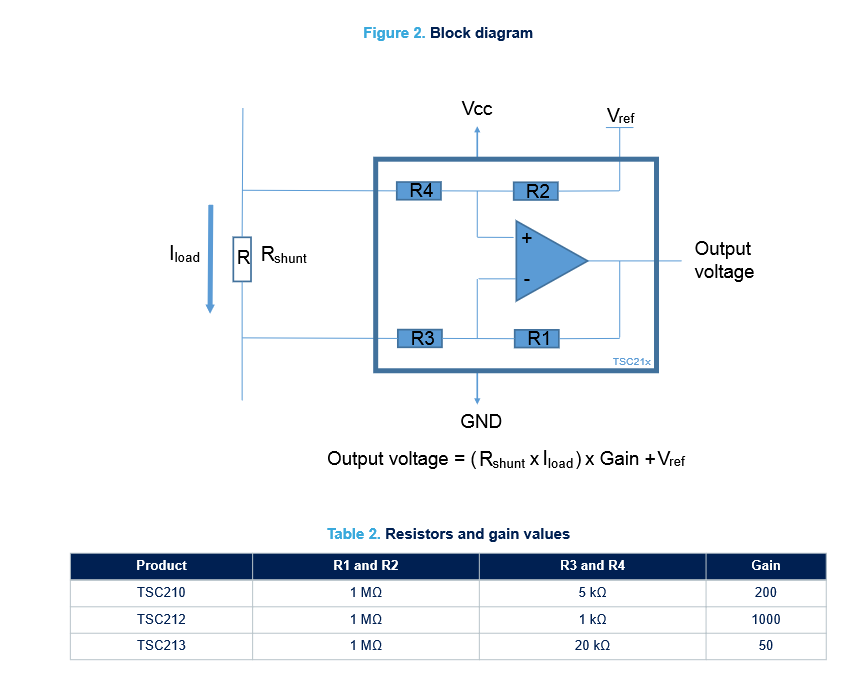
\includegraphics[scale=0.5]{./Figures/datasheet}
\caption{tsc213 data sheet information}
\label{fig:data}
\end{figure}


\begin{figure}[!htb]
\centering
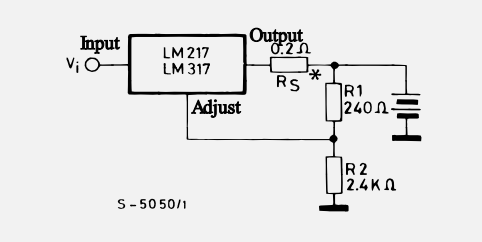
\includegraphics[scale=0.35]{Figures/circuitSTM.png}
\caption[Application Circuit For LM317]{Application Circuit For LM317\cite{STM}}
\label{fig:app}
\end{figure}




\begin{table}[!htb]
        \centering
        \footnotesize
        \caption[Thermal Resistance Values]{Thermal Resistance Values \cite{sink}\cite{STM}}
         \begin{tabular}{lrrrr}
          \toprule
             & $Thermal Resistance$ \\
             &  [\textdegree C/W] \\
          \midrule
          $\theta_{j-c}$ & 5      \\
          $\theta_{s-a}(worst case)$ &  20     \\
          $\theta_{j-a}$ &  50     \\

          \bottomrule
        \end{tabular}
     \label{tab:Thermal values}
\end{table}







\chapter{Hysterisis Calculations}
\begin{figure}[!htb]
	
\centering
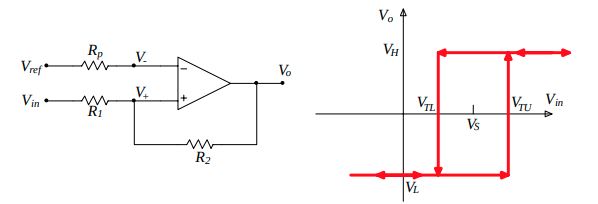
\includegraphics[scale=0.7]{./Figures/schmidt}
\caption[Non inverting Schmidt trigger]{Non inverting Schmidt trigger\cite{Schmidt}}
\label{fig:schmidt}
\end{figure}


For this analysis it will be assumed that we are working with an ideal op amp.
\begin{equation}
	V_+=V_-  
\end{equation}


Take a KCL at $V_+$ in figure \ref{fig:schmidt}:
\begin{equation}
	\frac{V_+-V_{in}}{R_1}+\frac{V_+-V_O}{R_2}=0
	\label{eq:kcl+}
	\end{equation}
		
		
Take a KCL at $V_-$ in figure \ref{fig:schmidt}:
\begin{equation}
	\frac{V_--V_{REF}}{R_p}=0
	\label{eq:kcl-}
\end{equation}

From equation \ref{eq:kcl-} the following result is achieved.
\begin{equation}
	V_-=V_{REF}
	\label{eq:kcl--}
\end{equation}


After rearranging eq. \ref{eq:kcl+} with $V_{in}$ as the subject. Also substitute \ref{eq:kcl--} into \ref{eq:kcl+}:

		\begin{equation}
V_{in}=\frac{V_{REF}\times (R_1+R_2)}{R_2}-\frac{V_{O}\times R_1}{R_2}
\end{equation}

The following two equations \ref{eq:vtl} and \ref{eq:vtu} are derived for the two scenarios where the output is at $V_H$ as well as $V_L$. At $V_H$ we want to find the voltage $V_{TL}$ where the the output will change rails to $V_L$. At $V_L$ we want to find the voltage $V_{TU}$ where the the output will change rails to $V_H$.:
\begin{equation}
	V_{TL}=\frac{V_{REF}\times (R_1+R_2)}{R_2}-\frac{V_{H}\times R_1}{R_2}
	\label{eq:vtl}
\end{equation}
	
	
	\begin{equation}
	V_{TU}=\frac{V_{REF}\times (R_1+R_2)}{R_2}-\frac{V_{L}\times R_1}{R_2}
	\label{eq:vtu}
\end{equation}

Now to achieve the following equation, subtract eq. \ref{eq:vtl} from eq. \ref{eq:vtu}:
\begin{equation}
		V_{TL}-V_{TU}=\frac{(V_{H}-V_L)\times R_1}{R_2}
			\label{eq:vtu-vtl}
	\end{equation}
		Rearrange eq. \ref{eq:vtu-vtl} to achieve the following equation:
		\begin{equation}
	\frac{V_{TL}-V_{TU}}{(V_{H}-V_L)}=\frac{R_1}{R_2}
\end{equation}

After calculating $\frac{R_1}{R_2}$ and therefore suitable resistors $V_{REF}$ can be found using the following equation. The following equation is obtained by making $V_{REF}$ the subject of equation \ref{eq:vtl}:

\begin{equation}
	V_{REF}=\frac{V_{TL}\times (R_2)}{R_1+R_2}+\frac{V_{H}\times R_1}{R_1+R_2}
	\label{eq:reff}
\end{equation}


%%%%%%%%%%%%%%%%%%%%%%%%%%%%%%%%%%%%%%%%%%%%%%%%%%%%%%%%%%%%%%%%%%%%%%%%%%%%%%%%%%%%%%%%%%%%%%%%%%%%%%%%%%%%%%%%%%%%%
\chapter{Differential amplifier calculations}
\begin{figure}[!htb]
	\centering
	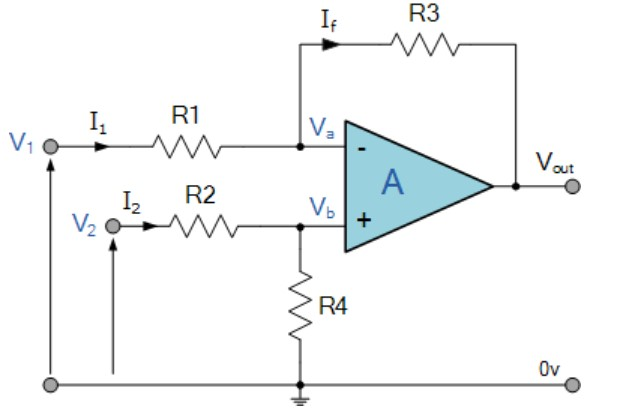
\includegraphics[width=0.4\linewidth]{Figures/A6/difamp.jpg}
	\caption[Differential amplifier op amp setup]{Differential amplifier op amp setup\cite{difAmp} }
	\label{fig:difamp2}
\end{figure}

\begin{figure}[!htb]
	\centering
	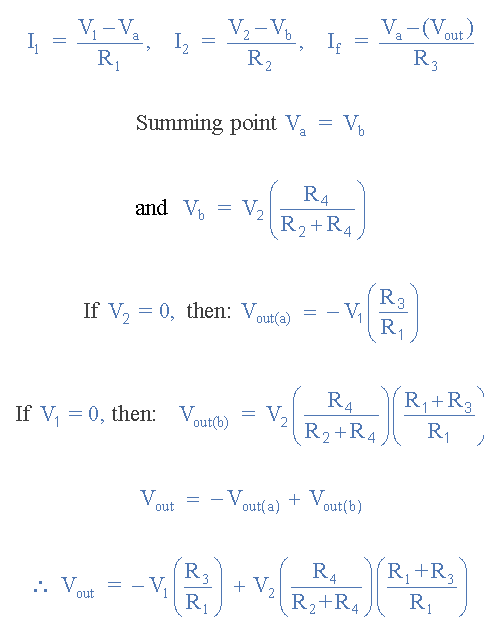
\includegraphics[width=0.4\linewidth]{Figures/A6/derive.png}
	\caption[Differential amplifier op amp setup derivation]{Differential amplifier op amp setup derivation\cite{difAmp} }
	\label{fig:derive}
\end{figure}


If $R_1=R_2$ and $R_3=R_4$ then the equation will simplify to :
\begin{equation}
	V_{out}=\frac{R_3}{R_1}\times(V_2-V_1)
\end{equation}

\chapter{Pilot LED calculations}

\label{appen:E}

\begin{figure}[!htb]
	\centering
	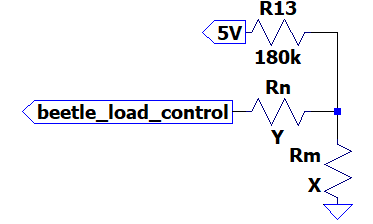
\includegraphics[width=0.2\linewidth]{Figures/A7/V-main.png}
	\caption{$V_-$ pilot LED calculations }
	\label{fig:v-main}
\end{figure}


$R_{13}$ is chosen to be 180k\textohm. When the load control is high the following equation can be found:
\begin{equation}
	3.5=\frac{R_m}{R_{n}||180k+R_m}
\end{equation}

\begin{equation}
	R_m=\frac{R_n\times 180k}{R_{n}+180k}\times \frac{3.5}{1.5}
	\label{eq:rm}
\end{equation}
\begin{figure}[!htb]
	\centering
	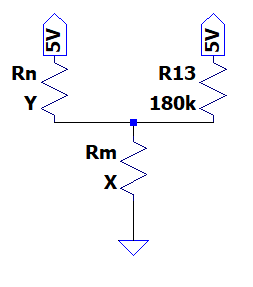
\includegraphics[width=0.2\linewidth]{Figures/A7/5Vv-.png}
	\caption{$V_-$ pilot LED calculations with load control on }
	\label{fig:v-5v}
\end{figure}



When the load control is low the following equation can be found:
\begin{equation}
	0.4=\frac{R_x}{R_x+180k}
\end{equation}
$R_x=15650$\textohm \\
Where $R_x$ is equal to $R_n$ in parallel with $R_m$:
\begin{equation}
	R_x=\frac{R_n\times R_m}{R_m+R_n}
	\label{eq:rx}
\end{equation}
\begin{figure}[!htb]
	\centering
	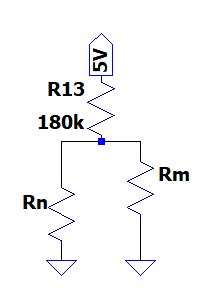
\includegraphics[width=0.2\linewidth]{Figures/A7/0Vv-.png}
	\caption{$V_-$ pilot LED calculations with load control off }
	\label{fig:v-0v}
\end{figure}

If eq.\ref{eq:rm} is substituted into eq. \ref{eq:rx} $R_n$ can be solved for: 

\begin{equation}
	15650=\frac{\frac{R_n\times 180k}{R_{n}+180k}\times \frac{3.5}{1.5}\times R_n}{\frac{R_n\times 180k}{R_{n}+180k}\times \frac{3.5}{1.5}+R_n}
\end{equation}
$R_n$=23.22k\textohm (lab resistor of 22k\textohm) \\
$R_m$=48k\textohm (lab resistor of 47k\textohm)


\chapter{Load control and pilot LED op amp voltages}

\label{appen:opamp}


\begin{table}[!htb]
	\centering
	\footnotesize
	\caption[Load Control circuit op amp requirements]{Load control and pilot LED circuit op amp requirements \cite{MCP}}
	\begin{tabular}{lrrrr}
		\toprule
		& $Min$ &$Max$&$Designed$ $range / value$\\
		&[V]&[V]&[V]\\
		\midrule
		All op amps Difference between supply rails $V_{DD} - V_{SS}$ & -& 7  &5   \\
		
		U1 Common mode voltage $(\frac{V_+ + V_-}{2}-V_{SS})$ &  -0.3&5.3&1.45-3\\
		U1 Differential Voltage $ (|V_+ - V_-|)$ & -& 5& 1-2.1  \\
		U1 Input voltages to $V_-$ and $V_+$  &  -1    &6&0.4-3.5 \\
		
		U2 Common mode voltage $(\frac{V_+ + V_-}{2}-V_{SS})$ &  -0.3&5.3&0-5\\
		U2 Input voltages to $V_-$ and $V_+$ &  -1    &6& 0-5 \\
		
		
		U3 Common mode voltage $(\frac{V_+ + V_-}{2}-V_{SS})$ &  -0.3&5.3&1.27-3.67\\
		U3 Input voltages to $V_-$ and $V_+$  &  -1    &6&0.03-4.85 \\
		U3 Differential Voltage $ (|V_+ - V_-|)$ & -& 5&  1-2.47  \\
		
		
		U4 Common mode voltage $(\frac{V_+ + V_-}{2}-V_{SS})$ &  -0.3&5.3&2.5-4.5\\
		U4 Input voltages to $V_-$ and $V_+$  &  -1    &6&0-4.5 \\
		U4 Differential Voltage $ (|V_+ - V_-|)$ & -& 5&  2.5-4.5  \\
		
		U5 Common mode voltage $(\frac{V_+ + V_-}{2}-V_{SS})$ &  -0.3&5.3&0.01-2.92\\
		U5 Input voltages to $V_-$ and $V_+$ &  -1    &6& 0.03-4.85 \\
		
		\bottomrule
	\end{tabular}
	\label{tab:MCPbat}
\end{table}

All op amps are within boundaries.

